\documentclass[12pt]{article}
\usepackage{setspace,graphicx,amsmath,geometry,fontspec,titlesec,soul,bm,subfigure}
\titleformat{\section}[block]{\LARGE\bfseries}{\arabic{section}}{1em}{}[]
\titleformat{\subsection}[block]{\Large\bfseries\mdseries}{\arabic{section}.\arabic{subsection}}{1em}{}[]
\titleformat{\subsubsection}[block]{\normalsize\bfseries}{\arabic{subsection}-\alph{subsubsection}}{1em}{}[]
\titleformat{\paragraph}[block]{\small\bfseries}{[\arabic{paragraph}]}{1em}{}[]
\setmainfont{Times New Roman}
\renewcommand{\baselinestretch}{1.15}
\renewcommand\contentsname{Inhaltverzeichnis}
\geometry{a4paper,left=2.5cm,right=2.5cm,top=2.5cm,bottom=2.5cm}
\begin{document}
	\newpagestyle{main}{            
		\sethead{Ziqing Yu}{Physikalische Geodäsie Übung 7}{3218051}     
		\setfoot{}{\thepage}{}     
		\headrule                                     
		\footrule                                       
	}
	\pagestyle{main}
\tableofcontents
\newpage
\section{Abschlussfehler}
Abschlussfehler der Höhendifferenz:
\begin{equation*}
\epsilon = \sum_{i} \Delta l_{i,i+1} = 0,0184 m
\end{equation*}
Abschlussfehler der Potentialdifferenz:
\begin{equation*}
\epsilon_W = \sum_{i} \Delta W_{i,i+1} = \sum_{i}\frac{g_i + g_{i+1}}{2} \Delta l_{i,i+1} = 0,1511 m^2/s^2
\end{equation*}
\section{Dynamische und Orthometrische Höhen}
Zuerst wird Normale Schwerkraft genutzt: $\gamma_{45} = 9,806199203 m/s^2$, die Höhe des erstes Punktes ist $436,52m$.
\begin{gather*}
\Delta l_{P_1 P_i} = \sum_{j=1}^{i-1} \Delta l_{P_j P_{j+1}} \\
DC_{P_1 P_{i}} = \sum_{j=1}^{i-1} \frac{\frac{g_j + g_{j+1}}{2} - \gamma_0}{\gamma_0} \Delta l_{P_j P_{j+1}} \\
\Delta H^d_{P_1 P_i} = \Delta l_{P_1 P_i} + DC_{P_1 P_{i}} \\
\end{gather*} 
Dynamische Höhe von erste Punkt $H_{P_1}^d = \frac{g_{P_1} + 0.0424 H^{O}_{P_1}}{\gamma_{45}} H^{O}_{P_1} = 436,62m$, dann haben wir: 
\begin{equation*}
H_{P_i}^{d} = H_{P_1}^{d} + \Delta H_{P_1 P_i}^d 
\end{equation*}
\begin{figure*}[ht]\centering
	\subfigure[Dynamische Höhen]{
		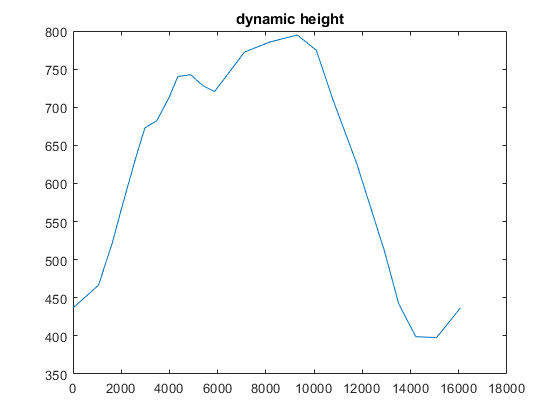
\includegraphics[width=0.5\textwidth]{dh.png}}
\end{figure*}
\newpage
Danach dürfen wir mit dynamische Höhen die Orthometrische Höhen rechnen:
\begin{equation*}
H_{P_i}^{O} = \frac{\gamma_{45}}{g_{P_i} + 0.0424(H^{O}_{P_i} + \sum_{j=1}^{i-1} \Delta P_j P_{j+1})} H^d_{P_i}
\end{equation*} 
\begin{figure*}[ht]\centering
	\subfigure[Orghometrische Höhen]{
		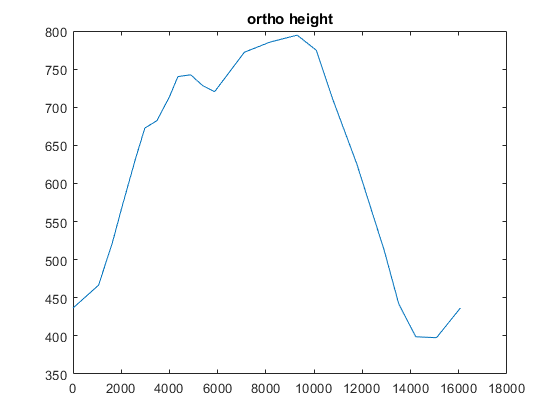
\includegraphics[width=0.5\textwidth]{oh.png}}
\end{figure*}
\newline
Die Formeln von Orthometrische Korrektion lautet:
\begin{equation*}
OC_{P_1 P_i} = DC_{P_1 P_i} + \frac{g_{P_1} + 0.0424 H^{O}_{P_1} - \gamma_{45}}{\gamma_{45}} H^{O}_{P_1} - \frac{g_{P_i} + 0.0424 H^{O}_{P_i} - \gamma_{45}}{\gamma_{45}} H^{O}_{P_i}
\end{equation*}
Die Darstellung von $DC$ und $OC$:
\begin{figure*}[ht]\centering
	\subfigure[Dynamische Korrektion]{
		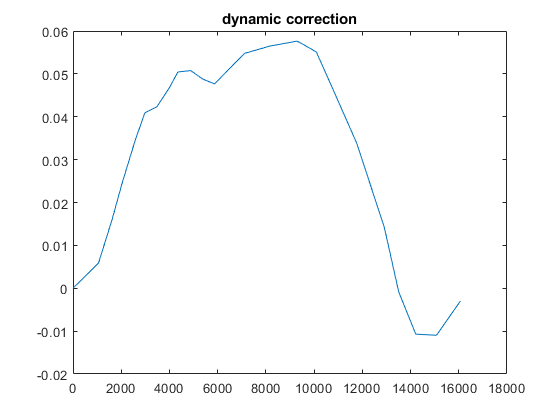
\includegraphics[width=0.45\textwidth]{dc.png}}
	\subfigure[Orghometrische Korrektion]{
		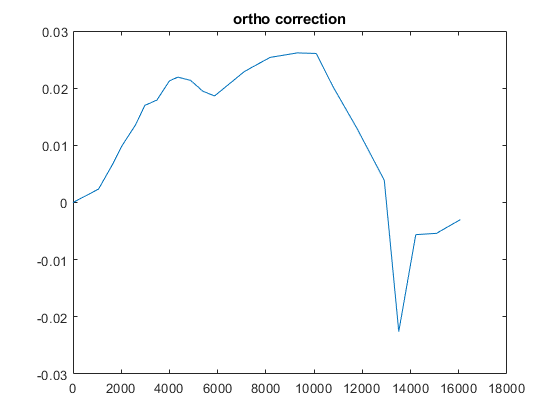
\includegraphics[width=0.45\textwidth]{oc.png}}
\end{figure*}
\newpage
Profil von Schwerkraft kann man auch zeichnen: 
\begin{figure*}[ht]\centering
	\subfigure[Schwerkraft]{
		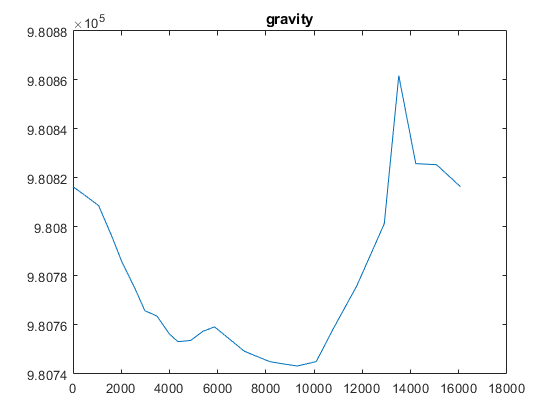
\includegraphics[width=0.5\textwidth]{g.png}}
\end{figure*}
\newline
Wenn wir $\gamma$ nicht $\gamma_{45} = 9,806199203 m/s^2$ sondern $\gamma_m = 9,797644656 m/s^2$ nehmen, sind die dynamische Korrektion anders:
\begin{figure*}[ht]\centering
	\subfigure[$\gamma_{45}$]{
		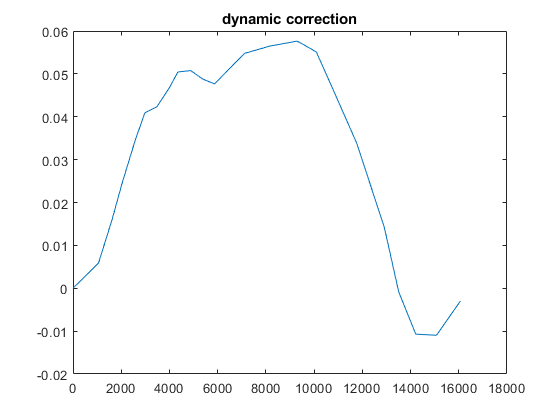
\includegraphics[width=0.45\textwidth]{dc.png}}
	\subfigure[$\gamma_m$]{
		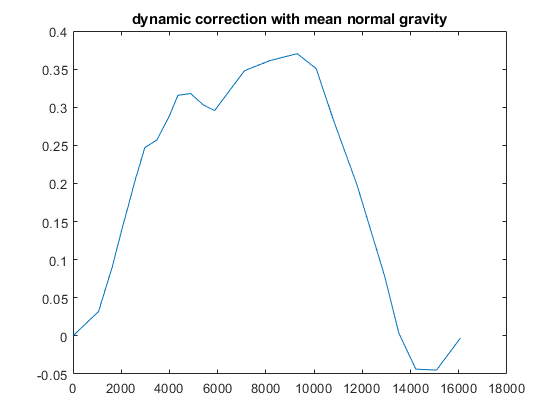
\includegraphics[width=0.45\textwidth]{dc2.png}}
\end{figure*}
\newline
Man kann deutlich sehen, dass die dynamische Korrektion viel größer wenn $\gamma$ kleiner ist, aber die Figur sehen ähnlich aus.
\end{document}